\chapter{Rotårsaksidentifisering}
Arbeidet i denne fasen går ut på å identifisere rotårsaken. I foregående fasen ble en rekke mulige årsaker identifisert og analysert, men nå er det tid for å finne den faktiske rotårsaken. Det er mange forskjellige verktøy som kan brukes i denne fasen, men vi har brukt et årsak-virkningsdiagram for vårt utgangspunkt.

\section{Årsak-virkningsdiagram}
Et årsak-virkning diagram er et diagram som analyserer forholdene mellom et problem og dets årsaker. Det kombinerer aspekter ved idémyldring med systematisk analyse. Det finnes to typer årsak-virkning diagrammer, fiskebeindiagram og prosessdiagram. Mens et prosessdiagram er mer direkte fokusert på problemet på innsiden av forretningsprosessene, er et fiskebeindiagram en mer generell tilnærming for å adressere alle potensielle årsaker\cite{RCA}. I dette caset har vi valgt et fiskebeindiagram på bakgrunn av at årsakene er spredt over flere variabler. 

\subsection{Ønsket utbytte}
Ved bruk av dette verktøyet ønsker vi å sitte igjen med en visuell fremstilling av rotårsakene til problemet. Dette vil gjøres ved å identifisere hva som skaper årsakene vi har funnet fram til i foregående fase. 

\subsection{Gjennomføring}
Det er anbefalt å bruke en tusjtavle for å tegne opp fiskebeindiagrammet, men vi valgte å bruke det nettbaserte programmet draw.io \cite{drawio}. Draw.io er laget for å skape diagrammer med flere brukere involvert i sanntid. De hadde en egen mal for fiskebeindiagram som vi valgte å gå ut fra. Stegene vi fulgte i prosessen er hentet fra boka om rotårsaksanalyse \cite{RCA} og ble som følger:

\begin{enumerate}
    \item Først ble problemet definert og skrevet i slutten av fiskebeindiagrammet.
    \item Deretter ble hovedkategoriene skrevet ned i bokser. Disse er direkte tilknyttet resultatene fra analysen.
    \item Videre startet vi å idémyldre alle mulige årsaker under hver kategori, en kategori om gangen. Disse ble fortløpende skrevet inn i diagrammet.
    \item Til slutt analyserte vi de identifiserte årsakene og bestemte de mest sannsynlige rotårsakene
\end{enumerate}

\subsection{Resultat}
Innledningsvis ble problemet beskrevet som rotårsaken til kompromitterte kontoer ved NTNU. Hovedkategoriene som ble undersøkt for å finne svar på dette, var gjenbruk av innloggingskredentialier tilhørende NTNU, IT-reglementet og andre styringsdokumenter, passordvaner, phishing og oversikt. Både hovedkategoriene og årsakene under disse er i hovedsak basert på dataanalysen, mens noe er basert på kreativ idémyldring. 

\begin{figure}[H]
    \centering
    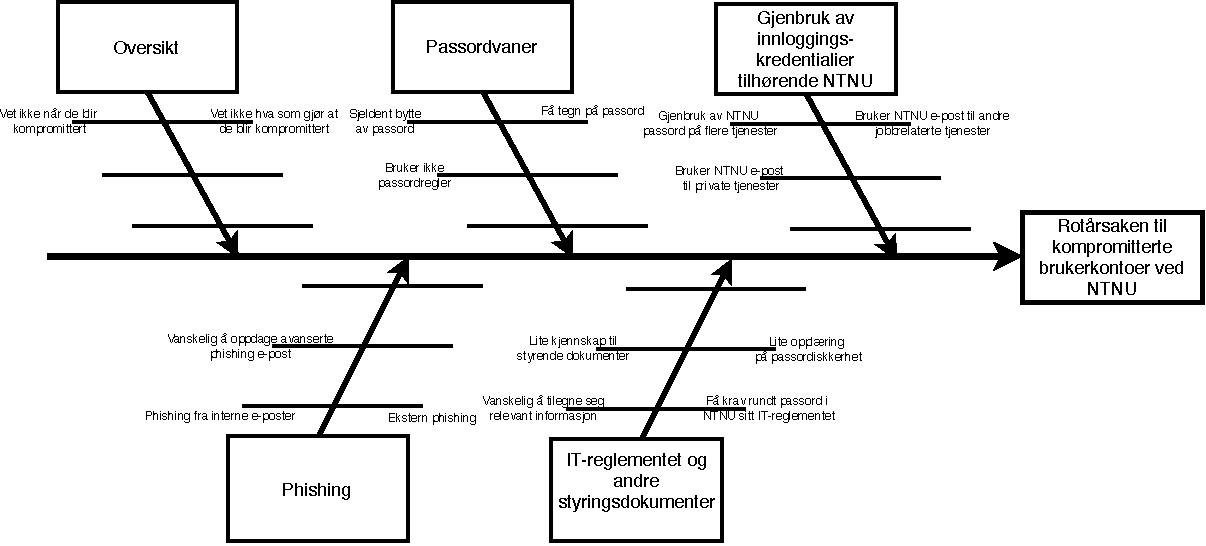
\includegraphics[scale=1.1, angle=90]{case_2/bilder/fiskebein.pdf}
    \label{fig:fiskebein-case2}
    \caption[Fiskebein-case2]{Fiskebeindiagram over hovedkategorier og årsaker}
\end{figure}

Vi har kommet frem til at rotårsaken til kompromitterte kontoer er sammensatt av flere faktorer. Et passord på mellom åtte til elleve tegn i seg selv er ikke nok for at kontoen skal bli kompromittert, men sammen med at de bytter sjeldnere enn hvert andre år gjør at dette blir et problem. I tillegg til dette bruker flertallet NTNU e-posten til andre tjenester, enten til jobbrelatert eller til privat bruk. De bruker også samme NTNU passord på flere tjenester. Dette er noe en burde unngå til enhver tid, og er noe av det vi anser å være blant det mest kritiske. 

Respondentene hadde også liten kjennskap til IT-reglementet og andre styringsdokumenter. De svarte også at de har fått lite opplæring på passordsikkerhet. Vi har lest igjennom IT-reglementet og andre styringsdokumenter, og har kommet frem til at IT-reglementet har for få krav til passord, det var vanskelig å tilegne seg all informasjon på de forskjellige styringsdokumentene da IT-reglementet ikke henviste til noen av retningslinjene. I Retningslinjer for behandling av brukernavn, passord og andre autentiseringsdata \cite{RetnBPA} står det at passordet skal byttes hver 12 måned. Denne retningslinjen er ikke nevnt i IT-reglementet at du skal gjøre deg bekjent med. 

Sammenlagt så viste det oss at respondentene hadde dårlige passordvaner, gjenbruk av innloggingskredentialier tilhørende NTNU og lite kunnskap til IT-reglementet og andre styrende dokumenter. Phishing er også en relevant årsak til kompromitterte kontoer. Phishing e-poster har blitt såpass sofistikerte at det er vanskelig å skille mellom falske og legimite e-poster. \cite{SophPhish}. Rotårsakene er derfor som følger: 

\begin{itemize}
    \item Mistet kontodetaljer av phishing
    \item E-post og passordgjenbruk på andre tjenester
    \item Liten kjennskap til IT-reglement og andre styrende dokumenter
    \item Dårlige passordvaner
\end{itemize}

\subsection{Konklusjon av verktøy}
Verktøyet fungerte veldig bra, siden det var så mange faktorer som kunne være rotårsakene. Det var litt vanskelig å gruppere hovedkategoriene i dette caset, fordi mange av årsakene kunne plasseres i flere hovedkategorier. Dette skyldes at problemet er spredt over flere årsaker som påvirkes av hverandre. Etter hovedkategoriene var definert var det enkelt å belyse årsaker, på grunn av gode data i dataanalysen. 

\section{5 Whys}
5 Whys er et verktøy som prøver å gjøre et dypdykk i årsakene for å finne rotårsaken. Måten dette gjøres på er å hele tiden spørre ``Why?'', altså hvorfor på norsk, hver gang en ny årsak dukker opp. Det brukes ofte for å sjekke om de identifiserte årsakene er symptomer, lav-nivå årsaker eller rotårsaker. 

\subsection{Ønsket utbytte}
Ved å bruke 5 Whys er det ønskelig å konfirmere om årsakene som ble fremhevet i fiskebeindiagrammet er faktiske rotårsaker, og ikke bare symptomer og/eller lav-nivå årsaker. 

\subsection{Gjennomføring}
Med dette verktøyet tar vi utgangspunkt i casebeskrivelsen, nemlig rotårsaken til kompromitterte kontoer ved NTNU. Ut fra dette brukte vi årsaker fra fiskebeindiagrammet over for å komme på årsaker som skal analyseres, samt prøvde å idémyldre et par nye. For hver av disse årsakene ble det spurt: ``Hvorfor er dette en årsak av det orginale problemet?''. For hvert svar spør vi hvorfor igjen og igjen helt til vi finner rotårsaken. Det ble tatt utgangspunkt i fem iterasjoner, men det er mulighet for flere eller færre avhengig av om spørsmålet kan besvares på en fornuftig måte. 

\subsection{Resultater}
Det ble fremhevet fem årsaker som skulle analyseres. Fire av disse kom fra fiskebeindiagrammet over, og en fra idémyldring. Tabellene under viser resultatene fra gjennomføringen. 

\begin{table} [H]
    \centering
    \begin{tabular}{ | m{5em} | m{30em} | }
        \hline
            \cellcolor{yellow} Årsak: & \cellcolor{yellow} Mistet kontodetaljer av phishing                \\
        \hline
            Why? & Fordi e-posten kom fra en intern e-postadresse                                   \\
        \hline
            Why? & Fordi kontoen var blitt kompomittert                                             \\
        \hline
            Why? & Fordi kontodetaljene ble phishet fra en ekstern e-postadresse                \\
        \hline
            Why? & Fordi brukeren var ikke oppmerksom på at det var en phishing e-post              \\
        \hline
            Why? & Fordi brukeren hadde ikke fått tilstrekkelig opplæring i deteksjon av phishing e-post    \\
        \hline
    \end{tabular}
    \caption[5 Whys: Mistet kontodetaljer av phishing]{5 Whys på mistet kontodetaljer av phishing}
    \label{5Whys-phishing}
\end{table}

Å miste kontodetaljer av en phishing e-post kan skje fra enten interne eller eksterne e-postadresser. I 5 Whys over kom vi frem til at dette skjer fordi en ikke er oppmerksom på tvilsomme e-poster. Årsaken til det kan være fordi brukerne ikke har fått tilstrekkelig opplæring i deteksjon av phishing e-post.

\begin{table} [H]
    \centering
    \begin{tabular}{ | m{5em} | m{30em} | }
        \hline
            \cellcolor{yellow} Årsak: & \cellcolor{yellow} E-post og passordgjenbruk på andre tjenester \\
        \hline
            Why? & Fordi det er vanskelig å huske mange unike brukerdetaljer \\
        \hline
            Why? & Fordi det ikke brukes passordmanager \\
        \hline
            Why? & Fordi de ikke vet hva det er \\
        \hline
            Why? & Fordi det ikke gis informasjon om det i retningslinjene \\
        \hline
            Why? & - \\
        \hline
    \end{tabular}
    \caption[5 Whys: E-post og passordgjenbruk på andre tjenester]{5 Whys på e-post og passordgjenbruk på andre tjenester}
    \label{5Whys-phishing}
\end{table}

Årsaken til at mange velger å benytte samme kredentialer flere steder er som regel at de synes det er vanskelig å huske mange brukerdetaljer, og motsatt, enkelt å huske få. Noe som kan gjøre dette lettere er å bruke en passordmanager, men dette informeres det ikke om i styringsdokumentene. 

\begin{table} [H]
    \centering
    \begin{tabular}{ | m{5em} | m{30em} | }
        \hline
            \cellcolor{yellow} Årsak: & \cellcolor{yellow} Liten kjennskap til IT-reglement og andre styrende dokumenter \\
        \hline
            Why? & Fordi det er vanskelig å tilegne seg informasjon \\
        \hline
            Why? & Fordi informasjonen er spredt på mange sider og dokumenter \\
        \hline
            Why? & Fordi det ikke er et overordnet ISMS \\
        \hline
            Why? & - \\
        \hline
            Why? & - \\
        \hline
    \end{tabular}
    \caption[5 Whys: Liten kjennskap til IT-reglement og andre styrende dokumenter]{5 Whys på liten kjennskap til IT-reglement og andre styrende dokumenter}
    \label{5Whys-phishing}
\end{table}

En mulig årsak til at det er liten kjennskap til disse dokumentene er at det er vanskelig å tilegne seg informasjonen. Det blir ofte mye for en person å forholde seg til, spesielt når informasjonen er spredt utover mange forskjellige sider og dokumenter. Et overordnet ISMS kunne hjulpet med å standardisere sikkerhetsstyringen, og kanskje sentralisere informasjonen. 

\begin{table} [H]
    \centering
    \begin{tabular}{ | m{5em} | m{30em} | }
        \hline
            \cellcolor{yellow} Årsak: & \cellcolor{yellow} Dårlige passordvaner \\
        \hline
            Why? & Fordi de er lite bevisste på sikkerhet \\
        \hline
            Why? & Fordi de tenker det ikke er så viktig \\
        \hline
            Why? & Fordi det er ingen tydelige krav rundt passord i NTNU sitt IT-reglement \\
        \hline
            Why? & Fordi IT-reglementet ikke henviser til de relevante dokumentene \\
        \hline
            Why? & - \\
        \hline
    \end{tabular}
    \caption[5 Whys: Dårlige passordvaner]{5 Whys på dårlige passordvaner}
    \label{5Whys-passordvaner}
\end{table}

Mange har dårlige passordvaner, fordi de er lite bevisste på sikkerhet, og at de ikke tenker det er så viktig. Mulig årsak til dette kan være fordi det ikke er noen tydelige krav rundt passord i NTNU sitt IT-reglement. IT-reglementet henviser ikke til de dokumentene som nevner passordrutiner \cite{ITReg}, og det er bare IT-reglementet brukerne er pliktig å sette seg inn i og skrive under på \cite{}. 

\begin{table} [H]
    \centering
    \begin{tabular}{ | m{5em} | m{30em} | }
        \hline
            \cellcolor{yellow} Årsak: & \cellcolor{yellow} Lukrativt for trusselaktører \\
        \hline
            Why? & Fordi de tjener og sparer penger på å kompromittere kontoer \\
        \hline
            Why? & Fordi de får tilgang til forskningsdatabaser \\
        \hline
            Why? & Fordi det er for enkelt å få tilgang til brukerkontoene \\
        \hline
            Why? & Fordi det er utilstrekkelig tilgangskontroll på brukerkontoene \\
        \hline
            Why? & - \\
        \hline
    \end{tabular}
    \caption[5 Whys: Lukrativt for datakriminelle]{5 Whys på lukrativitet for datakriminelle}
    \label{5Whys-passordvaner}
\end{table}

Det er lukrativt for datakriminelle å prøve å kompromittere brukerkontoer fordi det er for god kost-nytte effekt. De kan tjene penger på å selge kontoene, eller spare penger ved å laste ned forskningsartikler. Her kom vi frem til at utilstrekkelig tilgangskontroll kan være en rotårsak til at det er så høy kost-nytteverdi for trusselaktørene.

\subsection{Konklusjon av verktøy}
Verktøyet var svært nyttig for å gå dypt inn i årsakene. Et problem består ofte av flere nivåer av årsaker, og det tar 5 Whys hensyn til. I forhold til informasjonssikkerhet burde man passe på å ikke alltid ende opp med en årsak som er relatert til IT-reglementet eller andre styrende dokumenter, da problemet ofte også kan være av teknisk art. Et problem med verktøyet er at det kan bli for enssporet på en spesifikk tankegang. Det kan derfor anbefales i noen tilfeller å undersøke samme årsaken flere ganger dersom det er grunn til å tro at det finnes flere relevante årsaker ved ett av spørsmålene, som fører til en annen rotårsak. 




%Verktøyet var svært nyttig for å gå dypt inn i årsakene. Et problem består ofte av flere nivåer av årsaker, og det tar 5 Whys hensyn til. I forhold til informasjonssikkerhet burde man passe på å ikke alltid ende opp med en årsak som er relatert til Policy, da problemet ofte også kan være av teknisk art. Det var en mulig fallgruve for oss, men det er usikkert om det bare gjelder dette caset. Et annet problem med verktøyet er at det kan bli for enssporet på en spesifikk tankegang. Det kan derfor anbefales i noen tilfeller å undersøke samme årsaken flere ganger dersom det er grunn til å tro at det finnes flere relevante årsaker ved ett av spørsmålene, som fører til en annen rotårsak. 
